\section{Gráficos}
Nessa seção será apresentado todos os gráficos gerados a partir dos dados 
coletados. A análise dos dados será feita na seção 
\ref{sec:analise-dos-dados}.\\
Todos os gráficos foram gerados usando a ferramenta de geração de gráfico do 
\citeonline{LOcalc}.
% %GRAFICO 1
\subsection{Média do Tempo Total de Execução Dos Testes}

\begin{figure}[H]
	\centering
	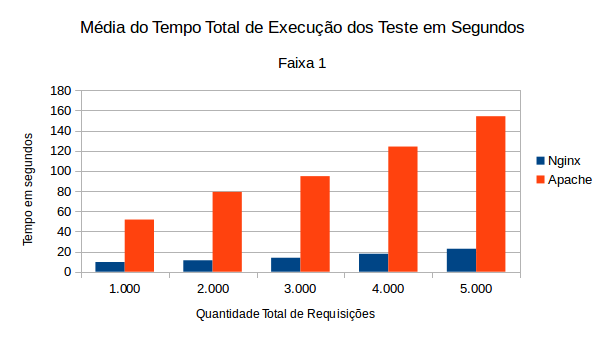
\includegraphics[width=1\linewidth]{graficos/grafico1-f1} 
	\caption{Média do Tempo Total de Execução dos Testes - Faixa 1}
	\label{fig:grafico1-f1}
\end{figure}

\begin{figure}[H]
	\centering
	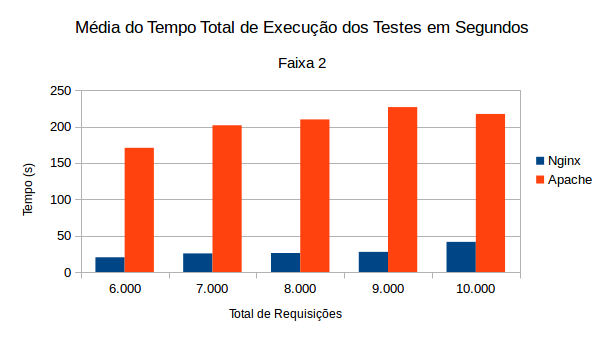
\includegraphics[width=1\linewidth]{graficos/grafico1-f2} 
	\caption{Média do Tempo Total de Execução dos Testes - Faixa 2}
	\label{fig:grafico1-f2}
\end{figure}

\begin{figure}[H]
	\centering
	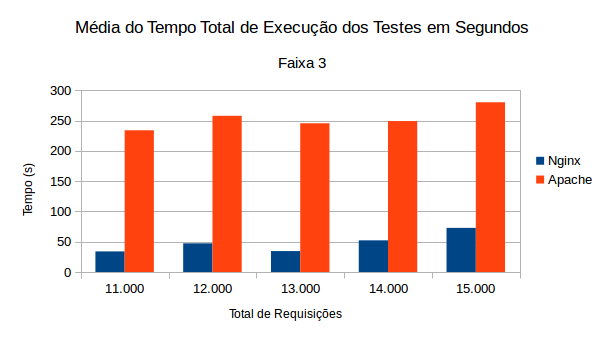
\includegraphics[width=1\linewidth]{graficos/grafico1-f3} 
	\caption{Média do Tempo Total de Execução dos Testes - Faixa 3}
	\label{fig:grafico1-f3}
\end{figure}

\begin{figure}[H]
	\centering
	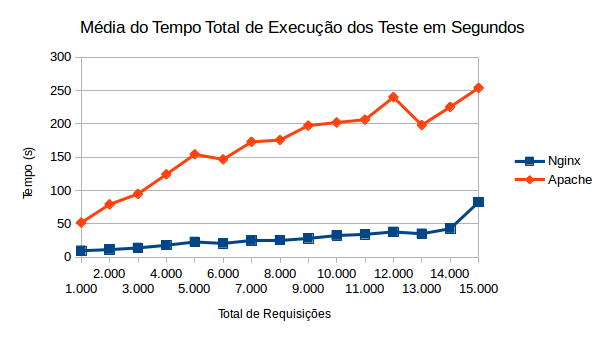
\includegraphics[width=1\linewidth]{graficos/grafico1} 
	\caption{Média do Tempo Total de Execução dos Testes}
	\label{fig:grafico1}
\end{figure}


% %GRAFICO 2
\subsection{Média do Total de Dados Transferido}
\begin{figure}[H]
	\centering
	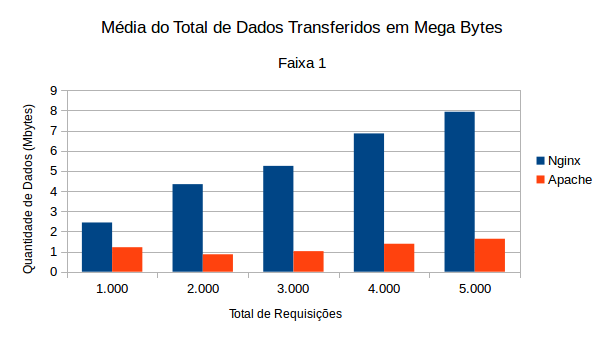
\includegraphics[width=1\linewidth]{graficos/grafico2-f1} 
	\caption{Média do Total de Dados Transferido - Faixa 1}
	\label{fig:grafico2-f1}
\end{figure}

\begin{figure}[H]
	\centering
	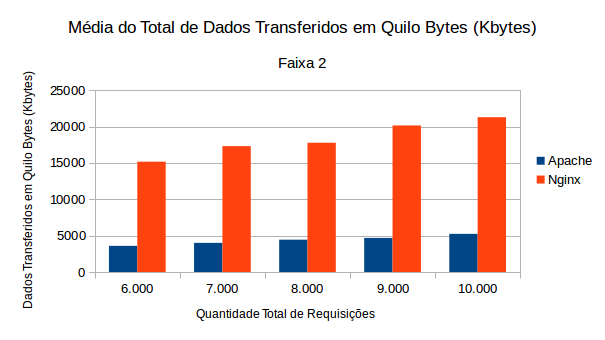
\includegraphics[width=1\linewidth]{graficos/grafico2-f2} 
	\caption{Média do Total de Dados Transferido - Faixa 2}
	\label{fig:grafico2-f2}
\end{figure}

\begin{figure}[H]
	\centering
	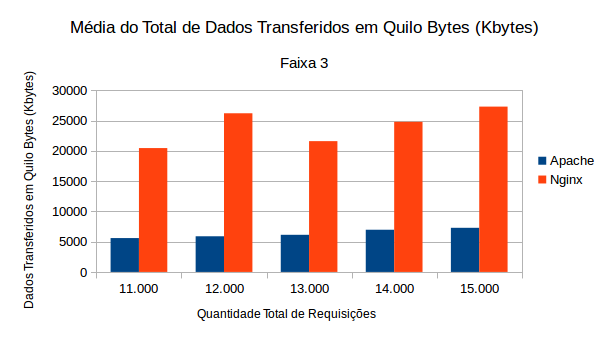
\includegraphics[width=1\linewidth]{graficos/grafico2-f3} 
	\caption{Média do Total de Dados Transferido - Faixa 3}
	\label{fig:grafico2-f3}
\end{figure}

\begin{figure}[H]
	\centering
	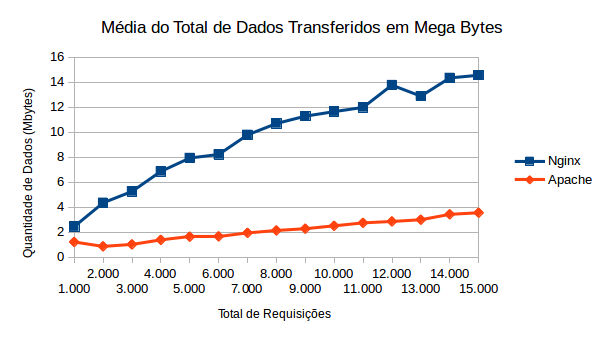
\includegraphics[width=1\linewidth]{graficos/grafico2} 
	\caption{Média do Total de Dados Transferido}
	\label{fig:grafico2}
\end{figure}

\begin{comment}
% %GRAFICO 3
\subsection{3}
\begin{figure}[htb]
	\centering
	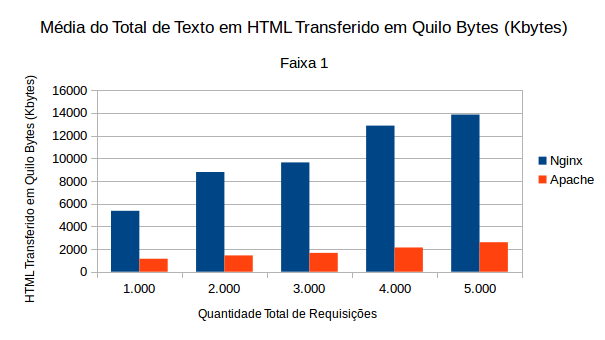
\includegraphics[width=1\linewidth]{graficos/grafico3-f1} 
	\caption{ - Faixa 1}
	\label{fig:grafico-f1}
\end{figure}

\begin{figure}[htb]
	\centering
	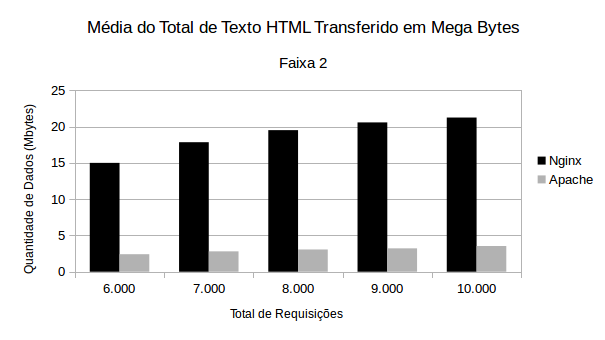
\includegraphics[width=1\linewidth]{graficos/grafico3-f2} 
	\caption{ - Faixa 2}
	\label{fig:grafico-f2}
\end{figure}

\begin{figure}[htb]
	\centering
	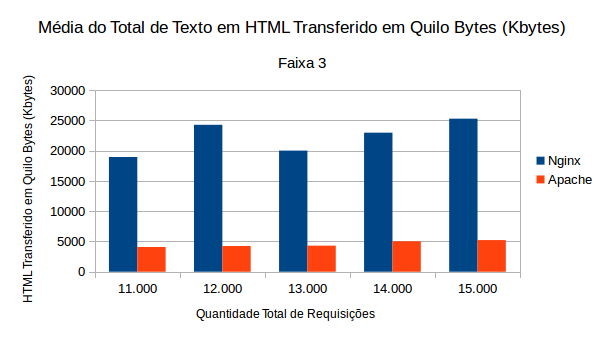
\includegraphics[width=1\linewidth]{graficos/grafico3-f3} 
	\caption{ - Faixa 3}
	\label{fig:grafico-f3}
\end{figure}

\begin{figure}[htb]
	\centering
	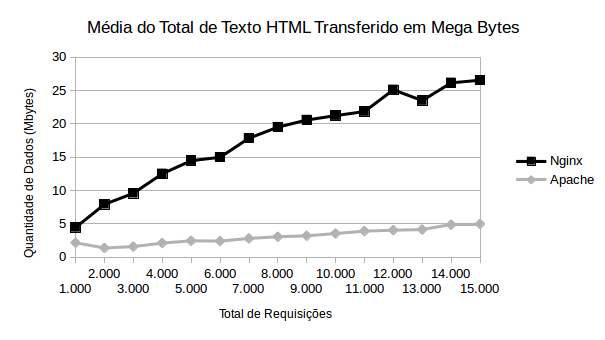
\includegraphics[width=1\linewidth]{graficos/grafico3} 
	\caption{}
	\label{fig:grafico}
\end{figure}
\end{comment}



